\chapter{Introduzione}

La gestione dinamica della memoria è una delle principali responsabilità dei sistemi operativi moderni\footnotemark. La memoria ospita i processi attivi e i dati correntemente elaborati dal \textit{software} in esecuzione; in quanto essa è più veloce da accedere dei dispositivi di memoria di massa, spesso viene usata come intermediario nella comunicazione che essi hanno con i processi. Con l'avvento dei sistemi multiprogrammati, la suddivisione della memoria in partizioni dedicate a ogni \textit{task} è diventata un aspetto principale dell'attività dei sistemi operativi: partizionare in aree contingentate la memoria in modo veloce ed efficiente (senza perdere tempo o sprecare memoria) è un compito sfidante. 
\footnotetext{Dove per memoria si intende la \textit{Random Access Memory}, o RAM.}

Il sistema operativo si deve occupare di gestire e monitorare lo stato di ciascuna locazione di memoria fisica, regolando l'allocazione della memoria tra i processi concorrenti, e definire le politiche di assegnazione, stabilendo quali processi possano accedere alla memoria, i tempi di allocazione e la quantità di memoria disponibile per ciascuno. Durante l'allocazione, il sistema operativo determina le specifiche locazioni di memoria da assegnare e ne mantiene traccia, aggiornandone lo stato in caso di rilascio o deallocazione. Un ulteriore aspetto che richiede attenzione è la memoria di cui il sistema operativo stesso ha necessità per svolgere le sue funzioni; poiché esso viene richiamato numerose volte dai programmi in esecuzione per svolgere molteplici compiti, laddove le strutture in atto per gestire le sue necessità di memoria siano lente o abbiamo un grande sovracosto ciò potrebbe portare a risultati disastrosi per la generale fluidità del calcolatore.

Quando la grandezza del programma è nota alla compilazione e non cambia, è semplice segnalare al sistema operativo quanta memoria sarà necessaria per tutto il ciclo di vita del programma. Questa memoria prende il nome di \textbf{staticamente allocata}. L'incarico di gestione risulta dunque semplificato: non sempre però è possibile determinare a priori le necessità del programma, in quanto queste potrebbero dipendere da vari fattori che non sono noti al programmatore (e.g. \textit{user input}). Un primo approccio, dispendioso e generalmente da evitare, consiste nell'allocare staticamente la memoria necessaria nel \textit{worst case scenario}. In questo modo però il sistema operativo potrebbe esaurire la memoria disponibile quando invece all'interno dei programmi esista memoria non utilizzata\footnotemark. In generale questa pratica risulta impossibile da applicare in contesti dove la quantità di memoria non è abbondante.

\footnotetext{Out of memory (OOM) error}

L'alternativa risulta immediata, ma non di facile implementazione: fornire al programmatore sistemi per \textbf{allocare dinamicamente} la memoria, ossia per variare la grandezza dell'area di memoria dedicata ai dati del programma durante la sua vita, ingrandendola e restringendola in base alle necessità. In questo modo, memoria viene occupata solamente quando è necessaria e nel momento in cui non è più utile viene restituita al sistema operativo, che può assegnarla a un altro programma. L'allocazione della memoria consiste dunque nell'identificare un blocco di memoria libera di dimensione adeguata per soddisfare una richiesta. Le allocazioni di memoria vengono gestite attingendo da un'area contigua denominata \textit{heap} (o \textit{free store}). 

\begin{figure}[H]
  \centering
  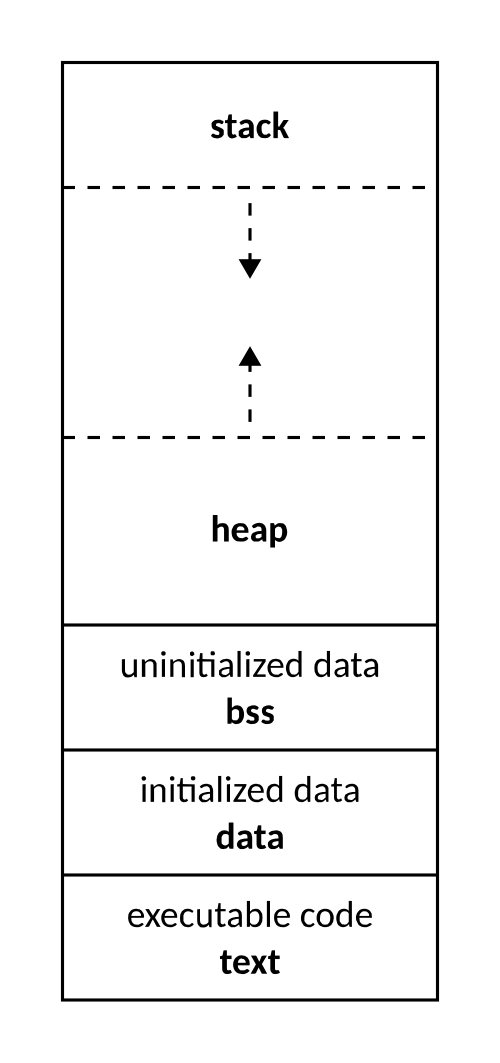
\includegraphics[width=0.2\textwidth]{images/program_memory_layout.png}
  \caption{Layout semplificato della memoria di un programma.}
  \label{fig:program_memory_layout}
\end{figure}

\section{\textit{Memory Allocators}}

In un dato istante, alcune regioni dell'\textit{heap} risultano allocate (in uso da parte di processi o strutture dati), mentre altre rimangono libere (non allocate) e pertanto disponibili per future richieste di memoria. Tale funzionalità è implementata da un modulo specializzato del sistema operativo, noto come \textit{Memory Allocator} (allocatore di memoria), il quale sovrintende all'assegnazione e al rilascio delle risorse di memoria. All'inizializzazione dell'allocatore viene riservata per il suo uso una quantità di memoria; esso si occupa dunque di gestirla dinamicamente, rispondendo alle necessità del programma e restituendo la memoria inutilizzata al sistema operativo. Ciò può avvenire secondo strategie e politiche ben diverse: obiettivo di questo progetto è l'esplorazione di un sottoinsieme rappresentativo di questi moduli, caratterizzati da un campione delle suddette politiche di allocazione, evidenziando nelle loro implementazioni i benefici e i punti deboli. 

Linguaggi di programmazione diversi gestiscono questa problematica in due modi: l'allocatore può funzionare in modo manuale, ossia rispondendo alla chiamata esplicita di funzioni che comunicano le necessità del programma, o in modo automatico, attraverso \textit{garbage collectors}. Questi ultimi consistono in un insieme di \textit{routine} che determinano se esiste memoria il cui riferimento viene perso all'interno del programma e che dunque sono irraggiungibili e li aggiungono alla memoria disponibile. Esistono diversi meccanismi per effettuare questa analisi, ma nel corso della nostra analisi ci concentreremo sull'allocazione manuale di memoria, in particolare nelle modalità in cui avviene nel linguaggio di programmazione \textbf{C}. 

La libC espone come interfaccia due primitive per l'allocazione di memoria: \textit{malloc} e \textit{free}. L'implementazione è lasciata al sistema operativo, che può decidere autonomamente quale tipologia di allocatore implementare, oppure addirittura di diversificare le strategie in base alle proprietà spaziali e temporali delle allocazioni.